\documentclass[tikz,border=10pt]{standalone}
\usepackage[utf8]{inputenc}
\usepackage{amsmath,amssymb}
\usepackage{tikz}
\usetikzlibrary{arrows,shapes,decorations.pathmorphing,positioning,3d}

\definecolor{geantblue}{RGB}{0,51,102}
\definecolor{leadgray}{RGB}{120,130,140}
\definecolor{airblue}{RGB}{230,240,250}

\begin{document}

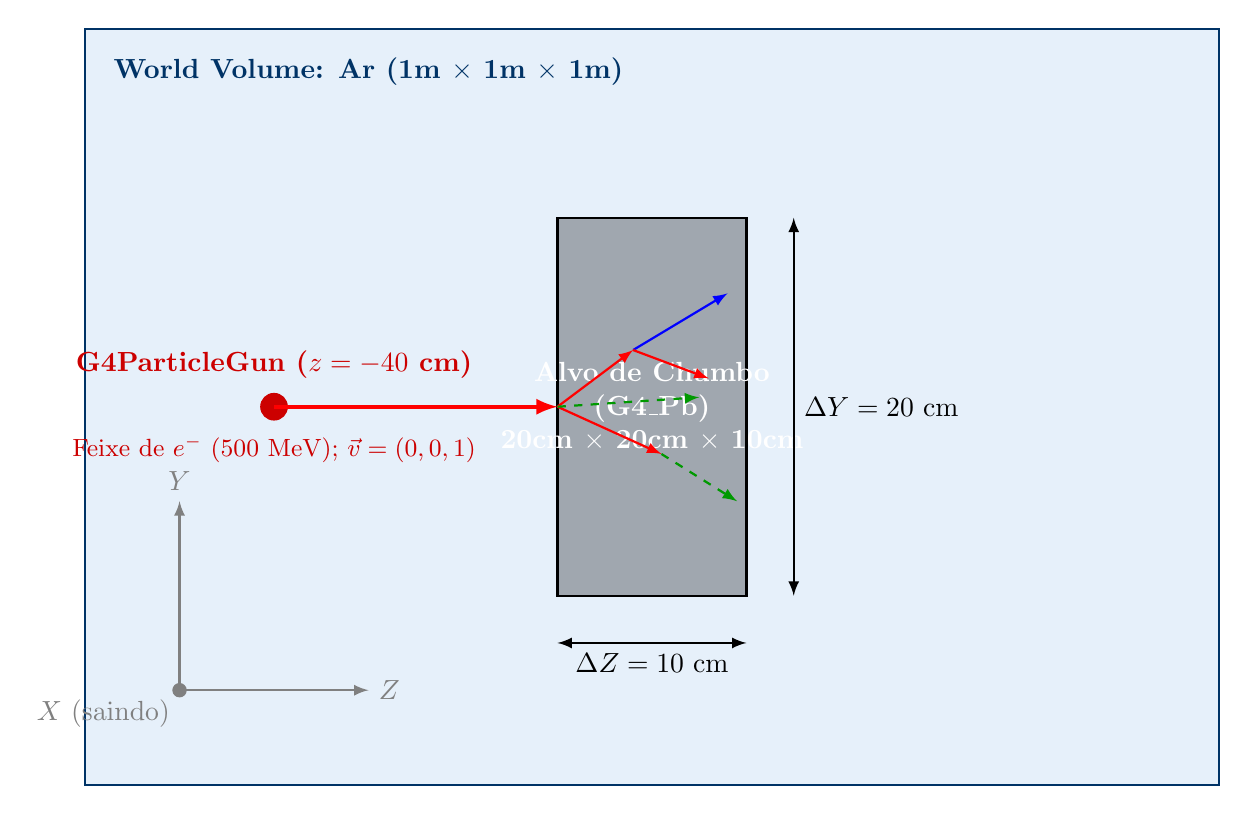
\begin{tikzpicture}[scale=1.2, >=latex]

    % 1. World Volume (1m x 1m, vista em corte 2D no plano Y-Z)
    \draw[thick, draw=geantblue, fill=airblue] (-6,-4) rectangle (6,4);
    \node[anchor=north west, geantblue, font=\bfseries] at (-5.8, 3.8) {World Volume: Ar (1m $\times$ 1m $\times$ 1m)};

    % 2. Eixos de Coordenadas
    \draw[->, thick, gray] (-5, -3) -- (-3, -3) node[right] {$Z$};
    \draw[->, thick, gray] (-5, -3) -- (-5, -1) node[above] {$Y$};
    \filldraw[gray] (-5, -3) circle (2pt) node[below left] {$X$ (saindo)};

    % 3. Alvo de Chumbo (20cm x 10cm no plano Z-Y)
    \draw[thick, draw=black, fill=leadgray!70] (-1.0, -2.0) rectangle (1.0, 2.0);
    \node[align=center, font=\bfseries, white] at (0, 0) {Alvo de Chumbo\\(G4\_Pb)\\20cm $\times$ 20cm $\times$ 10cm};

    % 4. Canhao de Particulas (Primary Particle Gun)
    \filldraw[red!80!black] (-4.0, 0) circle (4pt);
    \node[anchor=south, red!80!black, font=\bfseries] at (-4.0, 0.2) {G4ParticleGun ($z = -40\text{ cm}$)};
    \node[anchor=north, red!80!black, font=\small] at (-4.0, -0.2) {Feixe de $e^-$ ($500\text{ MeV}$); $\vec{v} = (0,0,1)$};

    % 5. Trajetoria da Particula Primaria e Chuveiro Eletromagnetico
    \draw[ultra thick, red, ->] (-4.0, 0) -- (-1.0, 0);

    % Chuveiro dentro do alvo
    \draw[thick, red, ->] (-1.0, 0) -- (-0.2, 0.6);
    \draw[thick, red, ->] (-1.0, 0) -- (0.1, -0.5);
    \draw[thick, green!60!black, dashed, ->] (-1.0, 0) -- (0.5, 0.1);
    \draw[thick, blue, ->] (-0.2, 0.6) -- (0.8, 1.2);
    \draw[thick, red, ->] (-0.2, 0.6) -- (0.6, 0.3);
    \draw[thick, green!60!black, dashed, ->] (0.1, -0.5) -- (0.9, -1.0);

    % 6. Cotas de Dimensoes
    \draw[<->, thick] (-1.0, -2.5) -- (1.0, -2.5) node[midway, below] {$\Delta Z = 10\text{ cm}$};
    \draw[<->, thick] (1.5, -2.0) -- (1.5, 2.0) node[midway, right] {$\Delta Y = 20\text{ cm}$};

\end{tikzpicture}

\end{document}
